\documentclass[8pt,a4paper]{article} % Compila con lualatex o xelatex

% --- Layout & links ---
\usepackage[margin=1.5in]{geometry}
\usepackage[hidelinks]{hyperref}

% --- Fuentes (texto y matemáticas) ---
\usepackage{newtxmath}
\usepackage{fontspec}
% \setmainfont{EB Garamond}[
%   UprightFont = * Medium,
%   ItalicFont = * Medium Italic,
%   BoldFont = * SemiBold,
%   BoldItalicFont = * SemiBold Italic
% ]
\setmainfont{EB Garamond}[
  UprightFont = * Regular,
  ItalicFont = * Italic,
  BoldFont = * SemiBold,
  BoldItalicFont = * SemiBold Italic
]

% --- Secciones y subsecciones ---
\usepackage{titlesec}
\newfontface\garamondbold{EB Garamond SemiBold}
\newfontface\garamondbolditalic{EB Garamond SemiBold Italic}
\titleformat{\section}
  {\garamondbold\Large}{\thesection}{1em}{}
\titleformat{\subsection}
  {\garamondbold\Large}{\thesubsection}{1em}{}

% --- Encabezado con nombre de la sección ---
\usepackage{fancyhdr}
\pagestyle{fancy}
\fancyhf{}
\fancyhead[L]{\small\leftmark}
\fancyhead[R]{\small\thepage}
\renewcommand{\headrulewidth}{0.0pt}

% --- Espaciado ---
\usepackage{setspace}

% --- Otros paquetes útiles ---
\usepackage{tocloft}  % Para personalizar la tabla de contenidos
\usepackage{xcolor}   % Para colores en el código
\usepackage{booktabs} % Para tablas bonitas
\usepackage{graphicx} % Para las graficas
\graphicspath{{../../../../visualizations/figuras/}}


% --- Código fuente ---
\usepackage{listings}
\lstset{
  basicstyle=\ttfamily\small,
  backgroundcolor=\color{gray!10},
  frame=single,
  breaklines=true
}


\usepackage{chngcntr}       % in preamble
\numberwithin{figure}{subsection}


\usepackage{lipsum}

\begin{document}

% --- Portada ---
\begin{titlepage}
  \centering
  \vspace*{4cm}
  {\Huge\bfseries CMAT\par}
  \vspace{2cm}
  {\Large Nombre del autor\par}
  \vspace{1cm}
  {\large Universidad de las Américas Puebla\par}
  \vfill
  {\large \today\par}
\end{titlepage}

% --- Resumen ---
\begin{abstract}
Este documento describe un flujo de análisis para evaluar la asociación entre el uso del CMAT (Centro de Matemáticas) y el desempeño académico, usando calificaciones estandarizadas (Z-score) con imputación de valores faltantes mediante KDE (Kernel Density Estimation). Se presentan: (i) exploración de la distribución de visitas, (ii) tratamiento e imputación de calificaciones, (iii) evidencia de heterogeneidad entre docentes, (iv) análisis por salón y por estudiante con pruebas paramétricas y no paramétricas, e (v) visualizaciones agregadas con intervalos de confianza.
\end{abstract}

% --- Tabla de contenidos ---
\tableofcontents
\thispagestyle{empty}
\newpage

% --- Inicio del documento ---
\section{Panorama general}
Este documento resume un análisis observacional del vínculo entre la frecuencia de visitas al CMAT y el desempeño en cursos, medido con calificaciones estandarizadas. 
Los enlaces como \href{https://example.com}{este} son activos.


\newpage
\section{\texorpdfstring{¿Qué es CMAT?}{Que es CMAT?}}
El CMAT (Centro de Matemáticas) es un espacio de asesorías académicas al que los estudiantes asisten para reforzar temas y resolver dudas. 
El objetivo analítico es comparar el desempeño de estudiantes con distinto nivel de uso del CMAT, evitando confundir efectos de calificación (p.ej., diferencias entre docentes) con cambios reales en desempeño.



\newpage
\section{Análisis exploratorio de datos}
Las Figuras 3.1.1 y 3.1.2 presentan la distribución del \textit{Número de Visitas} al CMAT por estudiante.
En la Figura 3.1.1 se muestra un histograma con eje $x$ en el rango $[0,120]$ visitas y eje $y$ ("Visitas") con conteos que alcanzan aproximadamente 7000.
La Figura 3.1.2 reutiliza el mismo histograma pero separa a los estudiantes en dos grupos por umbral de 3 visitas: "Más de 3 visitas" (9.95\%) y "3 o menos visitas" (90.05\%), lo que anticipa un diseño comparativo con fuerte desbalance de tamaños muestrales.

\subsection{\texorpdfstring{¿Cuántas personas fueron al CMAT?}{Cuantas personas fueron al CMAT?}}
En la Figura 3.1.1 el histograma de \textit{Número de Visitas} evidencia concentración en valores bajos (incluyendo 0) y una cola larga hasta alrededor de 120.
Los ejes están rotulados como "Número de Visitas" (horizontal) y "Visitas" (vertical), con marcas cada 20 visitas.
La Figura 3.1.2 introduce explícitamente la partición por frecuencia de uso del CMAT (más de 3 vs 3 o menos visitas) y reporta sus proporciones (9.95\% vs 90.05\%).

\begin{figure}[h]
    \centering
    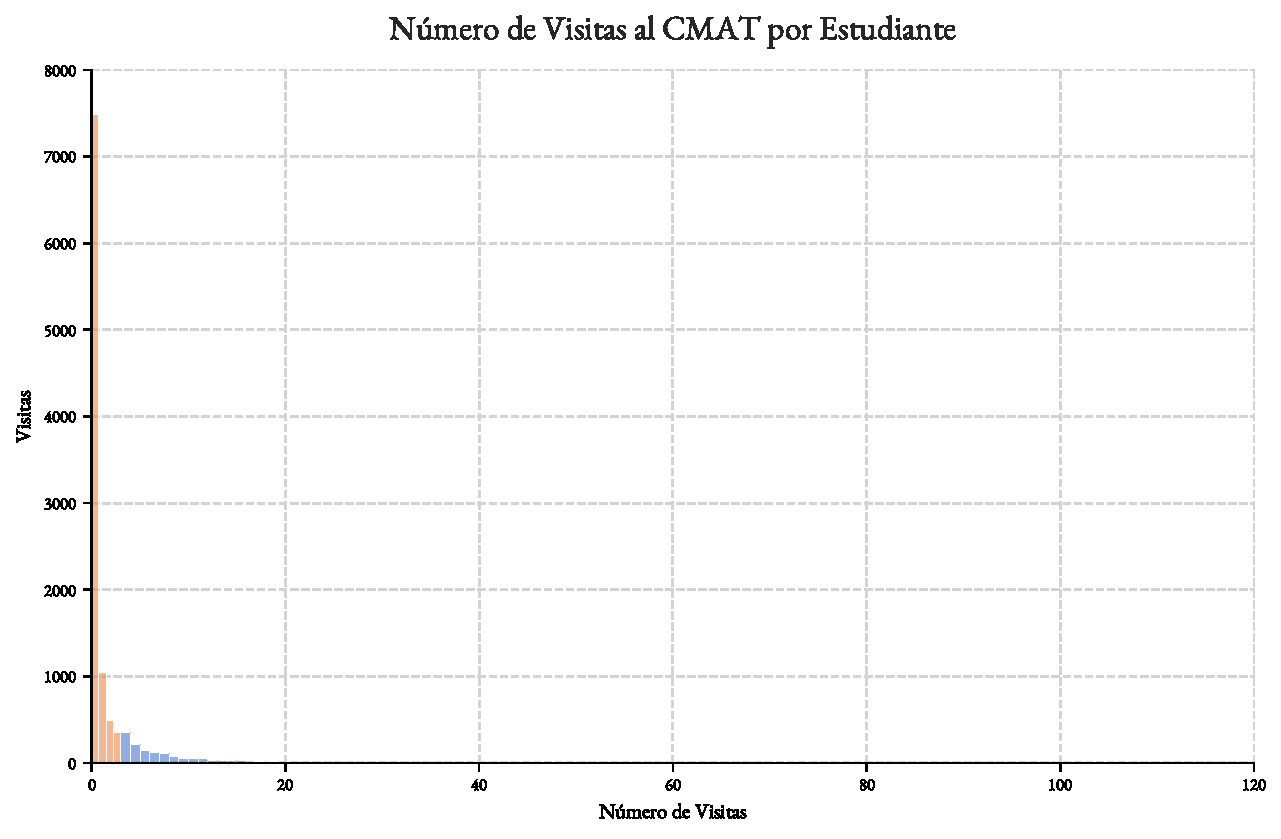
\includegraphics[width=0.7\textwidth,page=1]{03_01.pdf}
    \caption{Histograma del número de visitas al CMAT por estudiante.}
\end{figure}

\begin{figure}[h]
    \centering
    
\includegraphics[width=0.7\textwidth,page=1]{03_02.pdf}
    \caption{Histograma del número de visitas al CMAT con partición por umbral de 3 visitas (más de 3 vs 3 o menos).}
\end{figure}



\newpage
\section{\texorpdfstring{¿Mejoran su desempeño?}{Mejoran su desempeno?}}
Para operacionalizar la comparación de desempeño, la Figura 3.1.2 define el criterio de agrupamiento por visitas al CMAT (umbral $>3$).
En ese mismo gráfico se observa que el grupo de "Más de 3 visitas" representa 9.95\% frente a 90.05\% del grupo de "3 o menos visitas", por lo que cualquier contraste posterior debe considerar el desbalance.
El eje $x$ mantiene el rango aproximado $[0,120]$ visitas, consistente con el histograma base.

\subsection{\texorpdfstring{¿Cómo lo cuantificamos?}{Como lo cuantificamos?}}
La Figura 3.1.2 proporciona la variable explicativa (frecuencia de visitas) y la regla de corte (3 visitas) que se utilizará para comparar desempeño entre grupos.
El propio histograma con leyenda cuantifica los tamaños relativos (9.95\% vs 90.05\%), información necesaria para interpretar pruebas y estimadores que aparecen en figuras posteriores.
No se muestra en esta sección una figura adicional de desempeño; por tanto, la evidencia visual disponible aquí se restringe a la estratificación por visitas.

\subsection{\texorpdfstring{¿Con qué lo comparamos?}{Con que lo comparamos?}}
Sup: Con sus calificaciones.


\newpage
\section{Calificaciones}
En esta sección se documenta el tratamiento de calificaciones y su heterogeneidad mediante varias figuras.
La Figura 5.3.1 compara tres estrategias ante valores faltantes ("Eliminada", "Media" y "KDE") a partir de curvas de densidad sobre calificaciones en $[0,10]$.
Las Figuras 5.3.2--5.3.4 ilustran casos particulares (p.ej., rangos truncados y estandarización), mientras que las Figuras 5.3.5--5.3.6 muestran distribuciones agregadas por profesor, con proporciones de aprobados/reprobados reportadas en la propia gráfica.


\subsection{\texorpdfstring{¿Por qué hay valores faltantes?}{Por que hay valores faltantes?}}
Los estudiantes tienen la opción de no recibir calificación.

Sup: Los estudiantes evitan recibir calificación cuando anticipan que no aprobarán el curso.

\subsection{Imputación de valores faltantes}
En la Figura 5.3.1 se observa una comparación directa de métodos de imputación de calificaciones para un salón, con densidad en el eje $y$ y calificación en el eje $x$.
El gráfico superpone tres estimaciones identificadas en la leyenda como "Eliminada", "Media" y "KDE", permitiendo ver cómo cambia la forma de la distribución bajo cada manejo de faltantes.
El rango horizontal cubre de 0 a 10 y la escala de densidad llega aproximadamente a 0.35.


\subsection{\texorpdfstring{¿Son comparables las calificaciones?}{Son comparables las calificaciones?}}
La Figura 5.3.1 ("Comparación de Métodos de Imputación de Calificaciones para un Salón") sintetiza el impacto de eliminar registros vs imputar por media vs imputar por KDE.
Al compartir el mismo eje $x$ (0--10) y el mismo eje $y$ (densidad), el contraste es verificable visualmente por diferencias en alturas relativas y concentración de masa.
En ausencia de más anotaciones numéricas dentro del PDF, esta figura aporta principalmente evidencia descriptiva sobre la forma de las distribuciones generadas por cada método.

\begin{figure}[h]
    \centering
    
\includegraphics[width=0.7\textwidth,page=1]{05_01.pdf}
    \caption{Comparación de métodos de imputación de calificaciones para un salón: eliminación, imputación por media e imputación por KDE.}
\end{figure}

Casos especiales

\begin{figure}[h]
    \centering
    
\includegraphics[width=0.5\textwidth,page=1]{05_03.pdf}
    \caption{Distribución de calificaciones en un salón con valor atípico (vista acotada al rango 7.5--10).}
\end{figure}
La Figura 5.3.2 muestra la "Calificaciones de un Salón con un Valor Atípico" como una distribución de densidad restringida al intervalo 7.5--10.0.
El eje $y$ está rotulado como "Densidad" (0.0 a 1.0), lo que sugiere una concentración de observaciones en el tramo alto de la escala.
El hecho de que el eje $x$ comience en 7.5 es consistente con un caso donde no se observan calificaciones por debajo de ese umbral en ese salón.

\begin{figure}[h]
    \centering
    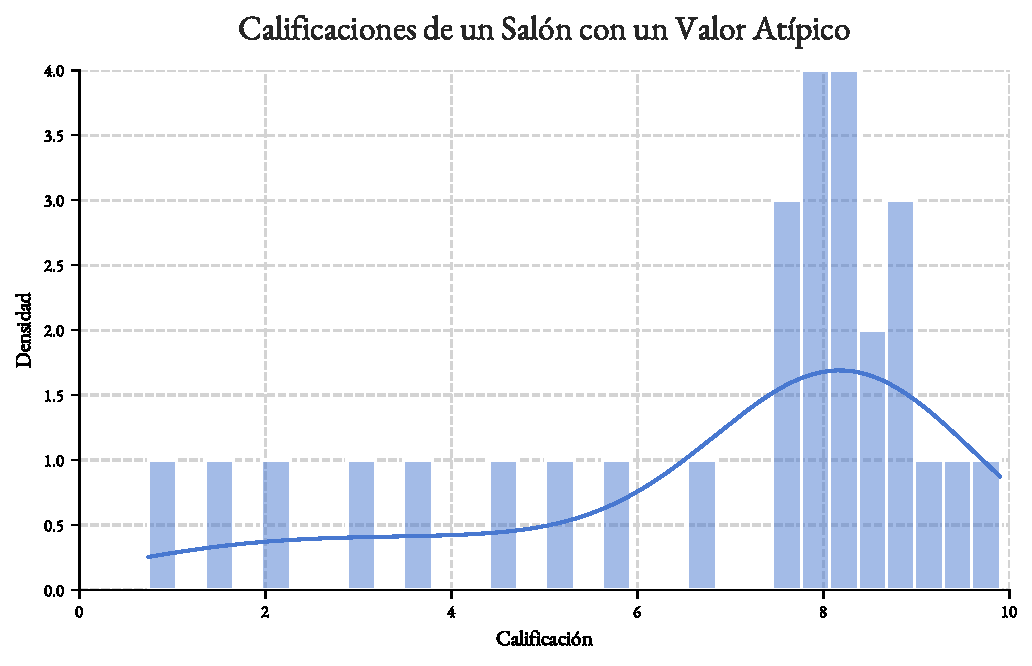
\includegraphics[width=0.5\textwidth,page=1]{05_04.pdf}
    \caption{Distribución de calificaciones en un salón con valor atípico (vista en el rango completo de calificación).}
\end{figure}
En la Figura 5.3.3 se representa nuevamente el caso de "Calificaciones de un Salón con un Valor Atípico", pero ahora sobre el rango completo de calificación (marcas en 2, 4, 6, 8, 10).
La escala de densidad alcanza aproximadamente 4.0, indicando picos más pronunciados que en la vista acotada de la Figura 5.3.2.
Esta visualización permite contrastar el comportamiento del mismo salón cuando se incluye el dominio completo de la variable.

\begin{figure}[h]
    \centering
    
\includegraphics[width=0.7\textwidth,page=1]{05_05.pdf}
    \caption{Comparación de métodos estandarizados de imputación (eliminación, media y KDE) sobre la escala de calificación.}
\end{figure}
La Figura 5.3.4 compara "Métodos Estandarizados de Imputación de Calificaciones" (Eliminada, Media, KDE) usando nuevamente curvas de densidad.
El eje $x$ recorre 0--10 y el eje $y$ (densidad) llega aproximadamente a 0.7, indicando que la estandarización cambia la escala de la estimación respecto a la Figura 5.3.1.
La leyenda hace explícitos los tres tratamientos de faltantes para evaluar su efecto en la distribución resultante.

\begin{figure}[h]
    \centering
    
\includegraphics[width=0.7\textwidth,page=1]{05_06.pdf}
    \caption{Distribución de calificaciones reportadas por profesor: densidades por docente y proporción de estudiantes.}
\end{figure}
En la Figura 5.3.5 se muestra la "Distribución de Calificaciones Reportadas por Profesor" como un conjunto de curvas de densidad por docente.
El gráfico incluye una barra/escala asociada a "Proporción de Estudiantes" y reporta tasas globales de "Reprobados: 9.43\%" y "Aprobados: 90.57\%".
Los ejes están definidos en calificación (0--10) y densidad, permitiendo comparar concentraciones y dispersión entre profesores.

\begin{figure}[h]
    \centering
    
\includegraphics[width=0.7\textwidth,page=1]{05_07.pdf}
    \caption{Distribución de calificaciones por profesor con imputación KDE: densidades por docente y proporción de estudiantes.}
\end{figure}
La Figura 5.3.6 presenta la "Distribución de Calificaciones por Profesor con Imputacion de KDE", incorporando el manejo de faltantes mediante KDE.
Se reportan explícitamente "Reprobados: 20.33\%" y "Aprobados: 79.67\%", junto con una escala de "Proporción de Estudiantes".
El eje horizontal es la calificación (0--10) y el eje vertical es densidad, mostrando la heterogeneidad de formas entre docentes tras la imputación.

\subsection{\texorpdfstring{¿Cómo califican los docentes a sus estudiantes?}{Como califican los docentes a sus estudiantes?}}
Las Figuras 5.4.1--5.4.8 exploran la heterogeneidad docente y su posible agrupamiento a partir de distribuciones de calificaciones.
En particular, la Figura 5.4.1 incorpora una matriz de estadísticos KS entre profesores (IMPKDE) y criterios de selección de $k$ para \textit{k-medoids} (método del codo y \textit{silhouette}).
Las Figuras 5.4.3--5.4.8 muestran distribuciones por profesor bajo imputación KDE, con distintas proporciones de reprobados/aprobados reportadas en cada gráfica.

\begin{figure}[h]
    \centering
    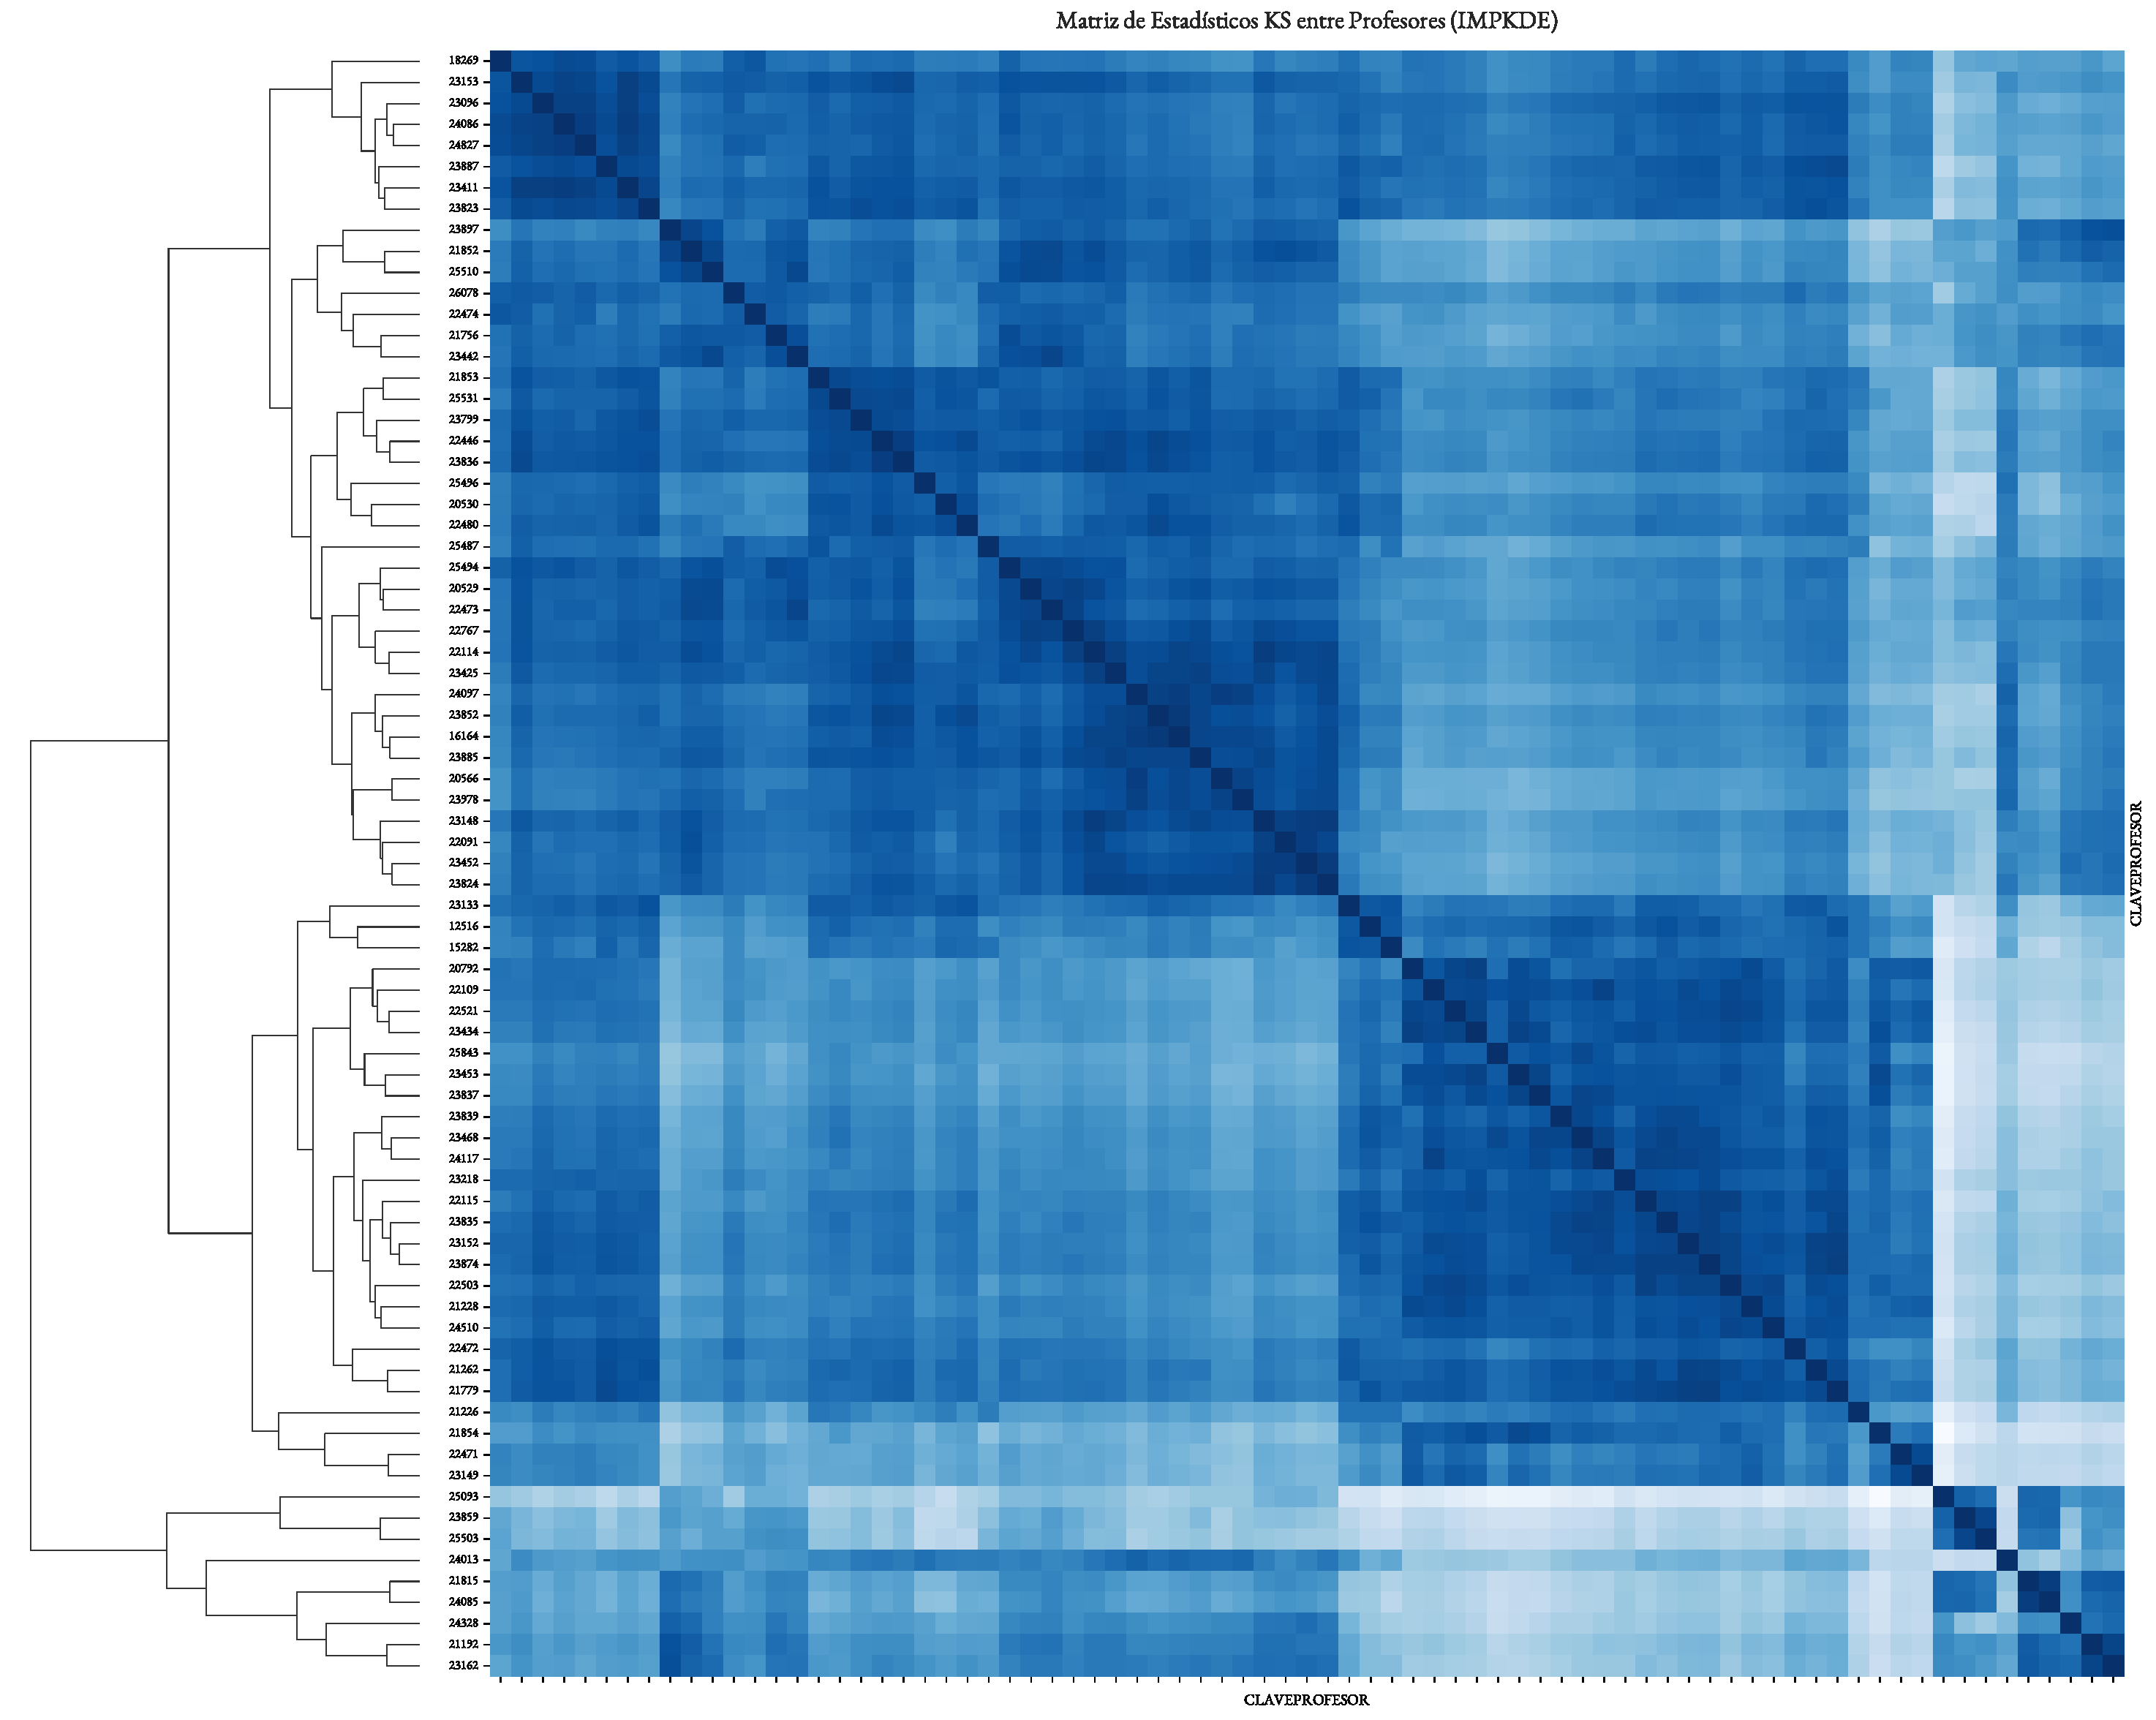
\includegraphics[width=0.7\textwidth,page=1]{05_08.pdf}
    \caption{Matriz de estadísticos KS entre profesores (IMPKDE) y criterios de selección de $k$ para \textit{k-medoids} (codo y \textit{silhouette}).}
\end{figure}
En la Figura 5.4.1 aparece la "Matriz de Estadísticos KS entre Profesores (IMPKDE)", con ejes rotulados como \texttt{CLAVEPROFESOR} y marcas identificadas por claves numéricas.
En el mismo entorno se incluyen dos diagnósticos para \textit{k-medoids}: "Elbow Method" (inercia vs número de clusters $k$) con anotación $k^*=3$, y "Silhouette Score" (silhouette vs $k$) con anotación $k^*=10$.
Ambos paneles usan $k$ en el rango 2--10, haciendo explícito el criterio de validación interna para el agrupamiento.

\begin{figure}[h]
    \centering
    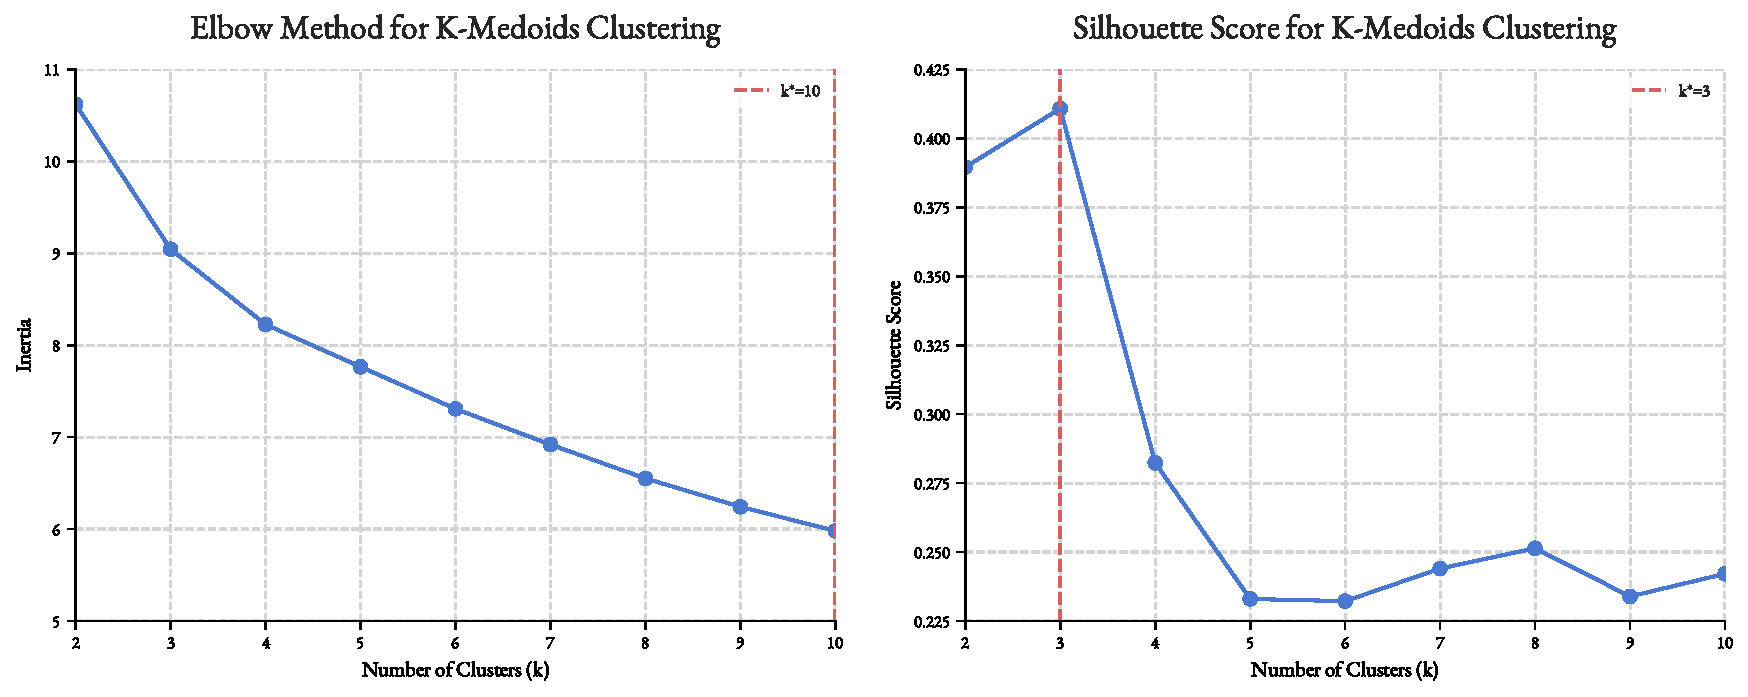
\includegraphics[width=0.7\textwidth,page=1]{05_09.pdf}
    \caption{Visualización complementaria asociada al análisis de heterogeneidad docente (detalles no legibles en el PDF).}
\end{figure}
En la Figura 5.4.2 no se extrae texto de títulos, ejes o leyendas desde el PDF, por lo que el contenido específico del gráfico no se distingue con claridad en esta conversión.
Únicamente es verificable su numeración (Figura 5.4.2) y su coexistencia temporal con la Figura 5.4.1 dentro del flujo del documento.
En consecuencia, cualquier interpretación adicional (p.ej., asignación de clusters o visualización de distancias) no puede afirmarse con certeza a partir del PDF disponible.

\begin{figure}[h]
    \centering
    
\includegraphics[width=0.7\textwidth,page=1]{05_10_0.pdf}
    \caption{Distribución de calificaciones por profesor con imputación KDE: escenario A (reprobados/aprobados según la anotación del panel).}
\end{figure}
La Figura 5.4.3 muestra "Distribución de Calificaciones por Profesor con Imputacion de KDE" con una escala de "Proporción de Estudiantes" y tasas: "Reprobados: 9.73\%" y "Aprobados: 90.27\%".
El eje $x$ es la calificación (0--10) y el eje $y$ es densidad, sugiriendo la superposición de múltiples curvas correspondientes a distintos profesores.
El propósito descriptivo es comparar la forma de las distribuciones docentes bajo el mismo esquema de imputación.

\begin{figure}[h]
    \centering
    
\includegraphics[width=0.7\textwidth,page=1]{05_10_1.pdf}
    \caption{Distribución de calificaciones por profesor con imputación KDE: escenario B (reprobados/aprobados según la anotación del panel).}
\end{figure}
En la Figura 5.4.4 se presenta nuevamente la "Distribución de Calificaciones por Profesor con Imputacion de KDE", ahora con "Reprobados: 17.16\%" y "Aprobados: 82.84\%".
El formato coincide con la Figura 5.4.3: calificación en 0--10, densidad en el eje vertical y una codificación asociada a la proporción de estudiantes.
La diferencia en la tasa reportada entre Figuras 5.4.3 y 5.4.4 es evidencia descriptiva de heterogeneidad agregada.

\begin{figure}[h]
    \centering
    
\includegraphics[width=0.7\textwidth,page=1]{05_10_2.pdf}
    \caption{Distribución de calificaciones por profesor con imputación KDE: escenario C (reprobados/aprobados según la anotación del panel).}
\end{figure}
La Figura 5.4.5 mantiene la misma estructura de visualización por profesor bajo imputación KDE, pero reporta "Reprobados: 32.89\%" y "Aprobados: 67.11\%".
Se observan los mismos ejes (calificación 0--10, densidad) y la referencia a "Proporción de Estudiantes".
Comparada con Figuras 5.4.3--5.4.4, esta gráfica documenta un escenario con mayor fracción de reprobación en el agregado mostrado.



\begin{figure}[h]
    \centering
    
\includegraphics[width=0.7\textwidth,page=1]{05_11_0.pdf}
    \caption{Distribución de calificaciones por profesor con imputación KDE: escenario D (reprobados/aprobados según la anotación del panel).}
\end{figure}
En la Figura 5.4.6 se vuelve a mostrar la distribución por profesor con imputación KDE, reportando "Reprobados: 9.73\%" y "Aprobados: 90.27\%".
El rango de calificación permanece en 0--10 y el eje vertical está en densidad, con codificación por proporción de estudiantes.
El hecho de que el porcentaje de reprobados coincida con el de la Figura 5.4.3 sugiere que ambas gráficas corresponden a subconjuntos distintos con métricas agregadas similares (no se identifica el criterio del subconjunto en el PDF).

\begin{figure}[h]
    \centering
    
\includegraphics[width=0.7\textwidth,page=1]{05_11_1.pdf}
    \caption{Distribución de calificaciones por profesor con imputación KDE: escenario E (reprobados/aprobados según la anotación del panel).}
\end{figure}
La Figura 5.4.7 repite la visualización de distribuciones por profesor con imputación KDE e indica "Reprobados: 17.16\%" y "Aprobados: 82.84\%".
Los ejes y la escala de proporción se mantienen, permitiendo comparar directamente con Figuras 5.4.4 y 5.4.5.
En el PDF no se distingue con claridad qué partición específica origina esta tasa, pero sí es verificable el valor reportado en la propia figura.

\begin{figure}[h]
    \centering
    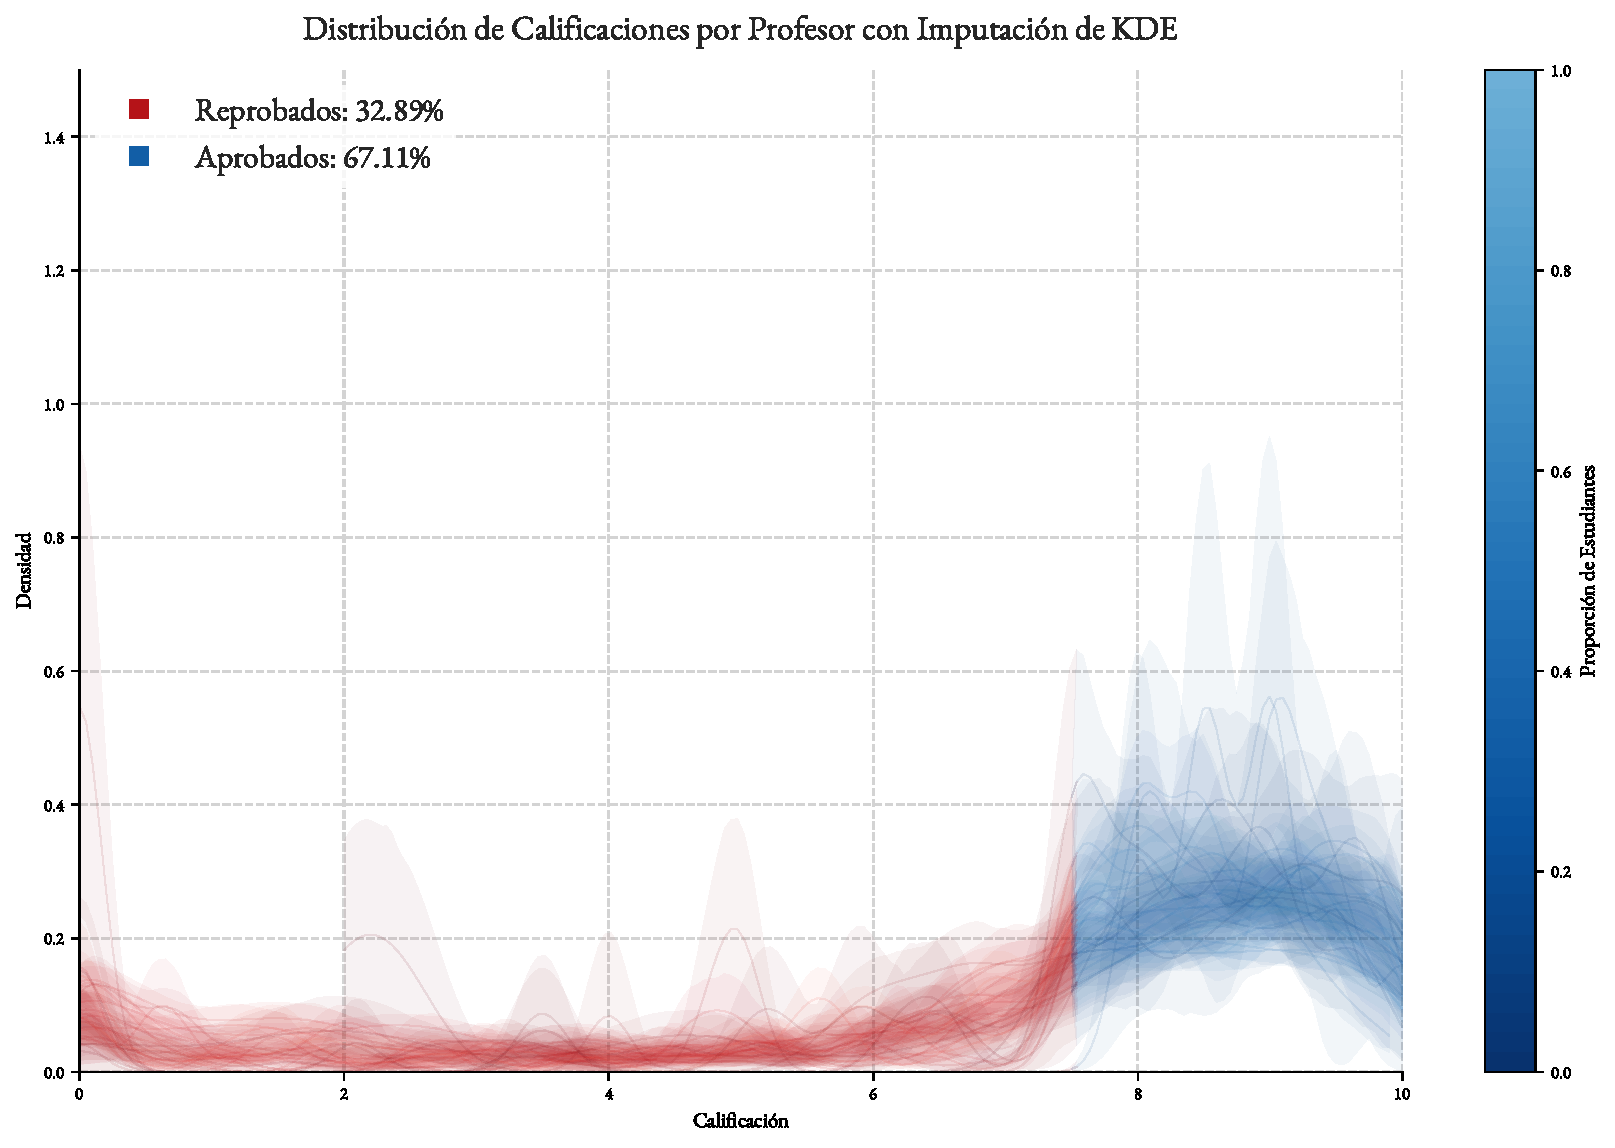
\includegraphics[width=0.7\textwidth,page=1]{05_11_2.pdf}
    \caption{Distribución de calificaciones por profesor con imputación KDE: escenario F (reprobados/aprobados según la anotación del panel).}
\end{figure}
En la Figura 5.4.8 se reporta nuevamente "Distribución de Calificaciones por Profesor con Imputación de KDE" con "Reprobados: 32.89\%" y "Aprobados: 67.11\%".
El diseño gráfico (calificación 0--10, densidad, escala de proporción de estudiantes) es consistente con Figuras 5.4.3--5.4.7.
Esta repetición de tasas (p.ej., 32.89\%) en diferentes figuras es consistente con comparaciones entre subconjuntos o agrupamientos, aunque el PDF no explicita el criterio en el propio panel.


Respuesta: se identifican múltiples patrones de calificación (p.ej., distribuciones con mayor concentración en valores altos vs escenarios con mayor masa bajo el umbral de reprobación).



\newpage
\section{\texorpdfstring{¿Cuál es la mejor forma de estandarizar?}{Cual es la mejor forma de estandarizar?}}
Esta sección aborda la estandarización de calificaciones, y la Figura 6.2.1 aporta evidencia temporal para un profesor específico.
En dicha figura se grafica la media de calificación por año (2019--2025) para el "Profesor 22471", con eje vertical "Media de Calificación" aproximadamente entre 5.5 y 8.5.
El objetivo descriptivo es mostrar variación longitudinal que puede requerir estandarización dependiente del tiempo.

\subsection{\texorpdfstring{Las calificaciones dependen del docente}{Las calificaciones dependen del docente}}
La Figura 6.2.1 (media anual por profesor) ilustra que el nivel de calificación puede depender del docente y variar entre años, incluso manteniendo la misma métrica (media).
El eje $x$ es el año (2019--2025) y el eje $y$ la media de calificación, con una trayectoria para el profesor identificado como 22471.
En el PDF no se distinguen valores puntuales por año, pero sí el rango vertical y la estructura temporal del gráfico.

\subsection{\texorpdfstring{Las calificaciones dependen del docente en el tiempo $t$}{Las calificaciones dependen del docente en el tiempo t}}
En la Figura 6.2.1 se presenta "Media de Calificaciones por Profesor a lo Largo de los Años" para el Profesor 22471.
El gráfico es una serie temporal con años 2019--2025 en el eje horizontal y "Media de Calificación" en el eje vertical (aprox. 5.5--8.5).
Este panel contextualiza la necesidad de considerar dependencia temporal ($t$) al comparar calificaciones entre cohortes.

\begin{figure}[h]
    \centering
    
\includegraphics[width=0.7\textwidth,page=1]{06_00.pdf}
    \caption{Media de calificaciones por profesor a lo largo de los años (serie temporal para el profesor mostrado en el panel).}
\end{figure}
La Figura 6.2.1 permite evaluar si la media anual del profesor 22471 se mantiene estable o fluctúa a lo largo de 2019--2025 dentro del rango mostrado (aprox. 5.5--8.5).
No se distingue con claridad en el PDF la dirección exacta de la tendencia (creciente/decreciente) ni los valores año a año.
Por tanto, la evidencia verificable aquí es la existencia de variación longitudinal potencialmente relevante para la estandarización.


\subsection{Entonces, por salón}

Se estandariza por salón (clase/aula).

Listo: esto establece una escala comparable (Z-score) dentro de cada salón, reduciendo el sesgo por diferencias sistemáticas entre docentes y cohortes.

\newpage
\section{Análisis por salón}
En el análisis por salón, las Figuras 7.0.1, 7.1.1 y 7.3.1 relacionan el número de visitas con la calificación estandarizada (KDE, Z-score).
La Figura 7.0.1 muestra un diagrama de dispersión visitas--Z-score por salón y separa visualmente los grupos "Más de 3 visitas" y "3 o menos visitas".
La Figura 7.1.1 añade una comparación de distribuciones con estadístico $t=24.34$ y $p$-valor 0.0000, mientras que la Figura 7.3.1 reporta pruebas no paramétricas, medianas y tamaños de efecto.

\begin{figure}[h]
    \centering
    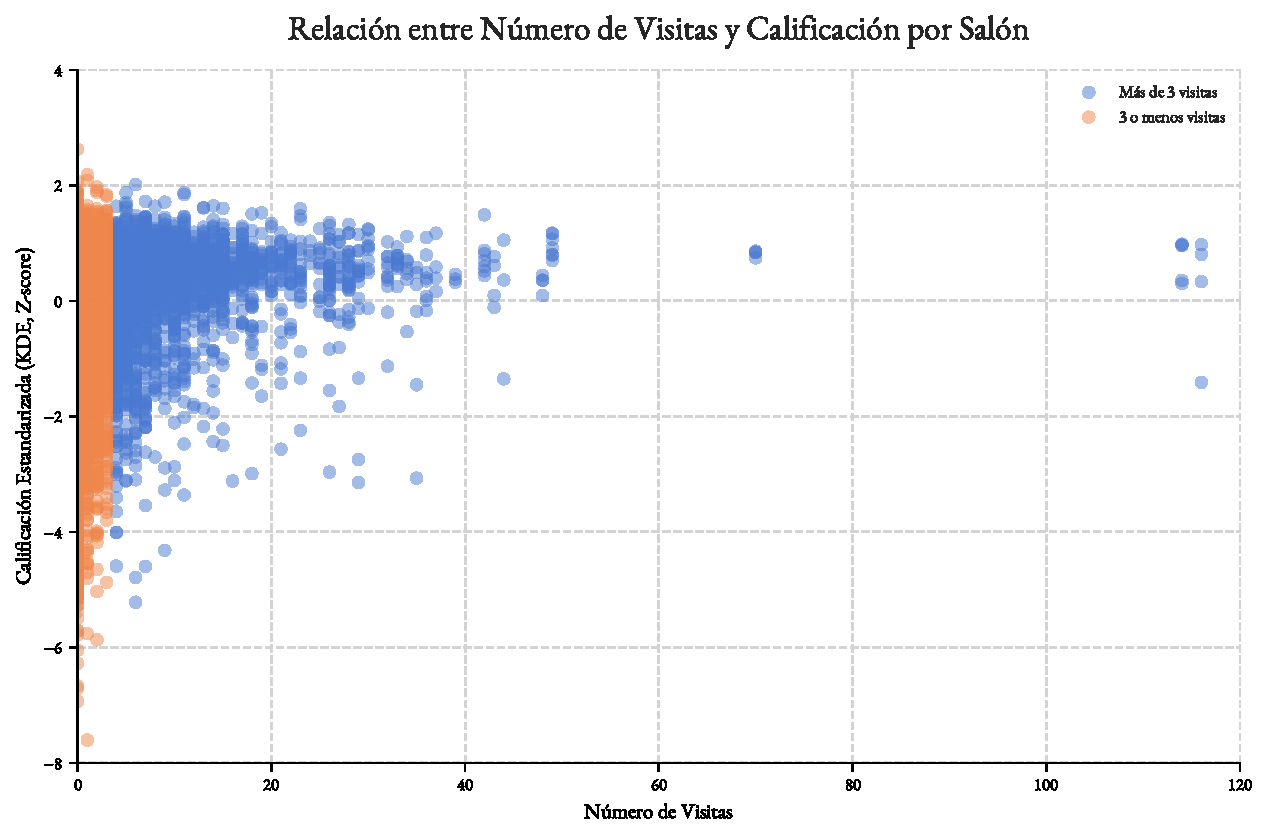
\includegraphics[width=0.7\textwidth,page=1]{07_00.pdf}
    \caption{Relación entre número de visitas y calificación estandarizada (KDE, Z-score) agregada por salón.}
\end{figure}
La Figura 7.0.1 ("Relación entre Número de Visitas y Calificación por Salón") es un diagrama de dispersión con "Número de Visitas" en el eje $x$ (0--120) y "Calificación Estandarizada (KDE, Z-score)" en el eje $y$.
La leyenda distingue dos grupos: "Más de 3 visitas" y "3 o menos visitas".
El gráfico permite inspeccionar visualmente la dispersión de Z-scores a distintos niveles de visitas sin implicar causalidad.

\subsection{Diferencia de medias}
La Figura 7.1.1 ("Comparación de Distribuciones de Calificaciones por Salón") muestra densidades para los dos grupos de visitas y reporta $t$-estadístico 24.34 con $p$-valor 0.0000.
El eje horizontal es la "Calificación Estandarizada (KDE, Z-score)" y el eje vertical es "Densidad".
En el panel se comparan las dos curvas etiquetadas como "Más de 3 visitas" y "3 o menos visitas".

\begin{figure}[h]
    \centering
    
\includegraphics[width=0.7\textwidth,page=1]{07_01.pdf}
    \caption{Comparación de distribuciones de calificación estandarizada por salón entre grupos de visitas (prueba $t$ reportada en el panel).}
\end{figure}
En la Figura 7.1.1 el contraste paramétrico se presenta como un resumen numérico (t=24.34, $p$=0.0000) junto a la superposición de densidades por grupo.
El rango del eje de Z-score incluye valores negativos y positivos, permitiendo apreciar diferencias de localización y dispersión entre grupos.
El PDF no muestra explícitamente las medias de cada grupo en este panel, por lo que la dirección del cambio debe inferirse de la posición relativa de las curvas.

\subsection{Intervalos de confianza}
Aunque esta subsección no incluye una figura exclusiva, los intervalos de confianza aparecen anotados en la Figura 7.3.1.
En particular, se reporta una diferencia de medianas "mediana = 0.205" con IC95\% [0.190, 0.224], junto con un $p$ de permutación para la mediana ($p_{\text{mediana}}=0.0003999$).
Estos elementos visuales conectan la cuantificación de incertidumbre con la comparación entre grupos por salón.

\subsection{Pruebas robustas}
La Figura 7.3.1 sintetiza pruebas no paramétricas y tamaños de efecto para la comparación por salón.
El panel reporta medianas por grupo (0.489 para "Más de 3 visitas" y 0.284 para "3 o menos visitas"), además de resultados de Mann--Whitney U ($p=4.958\times 10^{-117}$) y Brunner--Munzel ($p=9.599\times 10^{-122}$).
También incluye métricas de tamaño de efecto (CL=0.620, $r_{rb}=0.240$, Cliff's $\delta=0.243$) sobre el eje de calificación estandarizada.

\begin{figure}[h]
    \centering
    
\includegraphics[width=0.7\textwidth,page=1]{07_02.pdf}
    \caption{Comparación robusta por salón: densidades, medianas, pruebas no paramétricas y tamaños de efecto (anotados en el panel).}
\end{figure}
En la Figura 7.3.1 se detallan, en el propio gráfico, estimadores robustos: diferencia de medianas 0.205 con IC95\% [0.190, 0.224] y prueba de permutación para la mediana ($p_{\text{mediana}}=0.0003999$).
El panel incluye además CL=0.620 y $r_{rb}=0.240$, junto con Cliff's $\delta=0.243$, todos asociados a la comparación entre los dos grupos de visitas.
El eje $x$ es "Calificación Estandarizada (KDE, Z-score)" y el eje $y$ es densidad, por lo que las anotaciones se interpretan en la escala estandarizada.

\subsection{Intervalos de confianza}
La información de intervalos de confianza para el análisis por salón está integrada en la Figura 7.3.1, no en un panel separado.
Además del IC95\% para la diferencia de medianas, el gráfico reporta un valor puntual de mediana diferencial (0.205) y el $p$ de permutación asociado.
En el PDF no se distinguen bandas de confianza sobre la curva de densidad; la cuantificación de incertidumbre se presenta como texto anotado.

\subsection{Lectura descriptiva}
Para interpretación descriptiva por salón, la Figura 7.3.1 muestra que la mediana del grupo con más de 3 visitas (0.489) excede la del grupo con 3 o menos (0.284) en la escala Z.
Los $p$-valores extremadamente pequeños reportados (Mann--Whitney y Brunner--Munzel) respaldan una diferencia estadísticamente detectable entre distribuciones.
Sin embargo, la figura por sí sola no establece causalidad; únicamente documenta separación entre grupos definidos por visitas.


\newpage
\section{Análisis por estudiante}
El análisis por estudiante se resume visualmente en las Figuras 8.0.1, 8.1.1 y 8.3.1, todas en la escala "Calificación Estandarizada (KDE, Z-score)".
La Figura 8.0.1 muestra la relación visitas--Z-score por estudiante (dispersión), mientras que la Figura 8.1.1 compara densidades e incluye un contraste $t$ con medias y tamaños muestrales.
La Figura 8.3.1 añade un bloque de pruebas robustas (no paramétricas) con medianas, tamaños de efecto e intervalos de confianza.

\begin{figure}[h]
    \centering
    
\includegraphics[width=0.7\textwidth,page=1]{08_00.pdf}
    \caption{Relación entre número de visitas y calificación estandarizada (KDE, Z-score) a nivel estudiante.}
\end{figure}
La Figura 8.0.1 ("Relación entre Número de Visitas y Calificación por Estudiante") es un diagrama de dispersión con "Número de Visitas" en el eje $x$ (0--120) y Z-score estandarizado en el eje $y$.
La leyenda distingue "Más de 3 visitas" y "3 o menos visitas".
Esta figura permite contrastar la variabilidad individual frente al uso del CMAT, sin agregar por salón.

\subsection{Diferencia de medias}
En la Figura 8.1.1 ("Comparación de Distribuciones de Calificaciones por Estudiante") se reporta $t=21.93$ con $p$-valor 0.0000 y se declara la diferencia como estadísticamente significativa.
El gráfico anota las medias: 0.34 (más de 3 visitas) y -0.08 (3 o menos), con diferencia de medias 0.41.
También se reportan tamaños muestrales: $n=1036$ (más de 3) y $n=9377$ (3 o menos).

\begin{figure}[h]
    \centering
    
\includegraphics[width=0.7\textwidth,page=1]{08_01.pdf}
    \caption{Comparación de distribuciones de calificación estandarizada por estudiante entre grupos de visitas (prueba $t$, medias y $n$ anotados).}
\end{figure}
La Figura 8.1.1 incluye, además de las curvas de densidad por grupo, marcadores/etiquetas para las medias de cada grupo en la escala Z.
El resumen numérico (medias 0.34 vs -0.08; diferencia 0.41; $t=21.93$; $p$=0.0000) está impreso en el propio panel.
Esto permite una lectura verificable de dirección y magnitud del desplazamiento promedio entre grupos, a nivel estudiante.

\subsection{Intervalos de confianza}
Los intervalos de confianza relevantes para el análisis por estudiante se presentan como anotaciones en la Figura 8.3.1.
En esa figura se reporta CL=0.641 con IC95\% [0.625, 0.657] y $r_{rb}=0.282$ con IC95\% [0.250, 0.313].
También se incluye un IC95\% para la diferencia de medianas (0.237 con [0.202, 0.284]).

\subsection{Pruebas robustas}
La Figura 8.3.1 ("Comparación robusta de distribuciones por Estudiante") reporta medianas 0.422 (más de 3 visitas) y 0.185 (3 o menos visitas).
Se incluyen pruebas no paramétricas: Mann--Whitney U ($p=3.224\times 10^{-50}$) y Brunner--Munzel ($p=2.023\times 10^{-57}$), además de tamaños de efecto con intervalos de confianza.
El panel también presenta una prueba de permutación para la mediana con $p_{\text{mediana}}=0.0003999$.

\begin{figure}[h]
    \centering
    
\includegraphics[width=0.7\textwidth,page=1]{08_02.pdf}
    \caption{Comparación robusta por estudiante: densidades, medianas, pruebas no paramétricas, tamaños de efecto e IC95\% (anotados en el panel).}
\end{figure}
En la Figura 8.3.1 se muestran explícitamente CL=0.641 (IC95\% [0.625, 0.657]) y Cliff's $\delta=0.283$ (IC95\% [0.234, 0.326]).
La diferencia de medianas anotada es 0.237 con IC95\% [0.202, 0.284], junto con $r_{rb}=0.282$ (IC95\% [0.250, 0.313]).
Estas cantidades permiten comparar no solo significancia, sino tamaño de efecto entre grupos definidos por visitas, a nivel estudiante.

\subsection{Intervalos de confianza}
En ausencia de una figura separada para intervalos, la Figura 8.3.1 concentra la información de incertidumbre mediante IC95\% impresos para varios estimadores.
En particular, el IC95\% para la diferencia de medianas (0.237 con [0.202, 0.284]) y los IC95\% para CL y $r_{rb}$ están disponibles en el mismo panel.
El PDF no muestra bandas gráficas; los intervalos se reportan como texto anotado.


\newpage
\section{Gráfica agregada (``cute plot'')}
En la sección final de visualización se reutilizan gráficos del análisis por salón y se añade una agregación por número de visitas.
Las Figuras 9.0.1 y 9.1.1 replican, respectivamente, el diagrama de dispersión visitas--Z-score y la comparación de densidades con estadístico $t$.
La Figura 9.3.1 muestra el promedio de Z por salón contra número de visitas, incluyendo un intervalo de confianza del 95\%.

\begin{figure}[h]
    \centering
    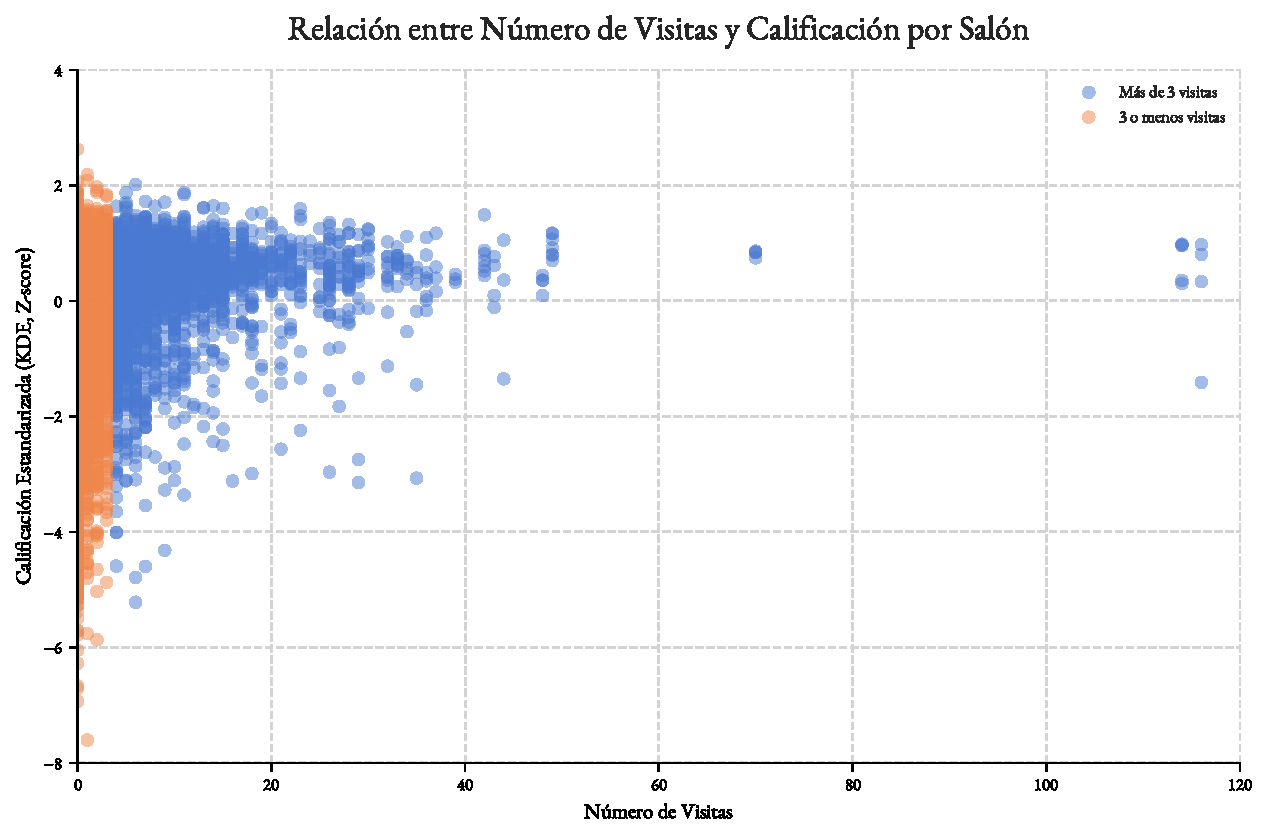
\includegraphics[width=0.7\textwidth,page=1]{07_00.pdf}
    \caption{Relación entre número de visitas y calificación estandarizada (KDE, Z-score) por salón (reutilizada como referencia).}
\end{figure}
La Figura 9.0.1 muestra "Relación entre Número de Visitas y Calificación por Salón" con "Calificación Estandarizada (KDE, Z-score)" en el eje $y$ y "Número de Visitas" en el eje $x$.
Se distinguen dos grupos (más de 3 visitas vs 3 o menos visitas) mediante la leyenda.
El rango horizontal llega a aproximadamente 120 visitas, permitiendo ver el comportamiento en la cola de uso intensivo.

\subsection{Diferencia de medias}
La Figura 9.1.1 (``Comparación de Distribuciones de Calificaciones por Salón'') superpone densidades de Z-score para ambos grupos y reporta $t=24.34$ con $p$-valor 0.0000.
El eje $x$ está en ``Calificación Estandarizada (KDE, Z-score)'' y el eje $y$ en densidad.
El panel permite una lectura directa de la diferencia detectada por la prueba $t$ junto con la forma de las distribuciones.

\begin{figure}[h]
    \centering
    
\includegraphics[width=0.7\textwidth,page=1]{07_01.pdf}
    \caption{Comparación de distribuciones por salón entre grupos de visitas (reutilizada como referencia; prueba $t$ reportada en el panel).}
\end{figure}
En la Figura 9.1.1, el resultado paramétrico (t=24.34, $p$=0.0000) aparece como texto en el mismo gráfico de densidades.
Las curvas están etiquetadas por grupo de visitas, facilitando la comparación visual en la escala estandarizada.
No se distinguen en el PDF valores de media explícitos en este panel; la interpretación se apoya en la superposición de densidades y el estadístico reportado.

\subsection{Intervalos de confianza}
Los intervalos de confianza en esta sección se visualizan principalmente en la Figura 9.3.1.
Ahí se muestra la serie ``Media Z por visitas'' y se incluye explícitamente ``IC 95\%'' como banda o barras alrededor de la media agregada.
Por tanto, la cuantificación de incertidumbre está asociada a la relación promedio Z--número de visitas, no a las densidades de la Figura 9.1.1.

\subsection{Agregación con incertidumbre}
La Figura 9.3.1 (``Z Promedio por Salón vs Número de Visitas'') grafica la ``Media de Z'' en función del ``Número de visitas''.
El panel incluye dos elementos en la leyenda: la media (``Media Z por visitas'') y su ``IC 95\%''.
El eje $x$ cubre aproximadamente 0--30 visitas y el eje $y$ muestra medias de Z en el rango aproximado [-0.5, 1.5].

\begin{figure}[h]
    \centering
    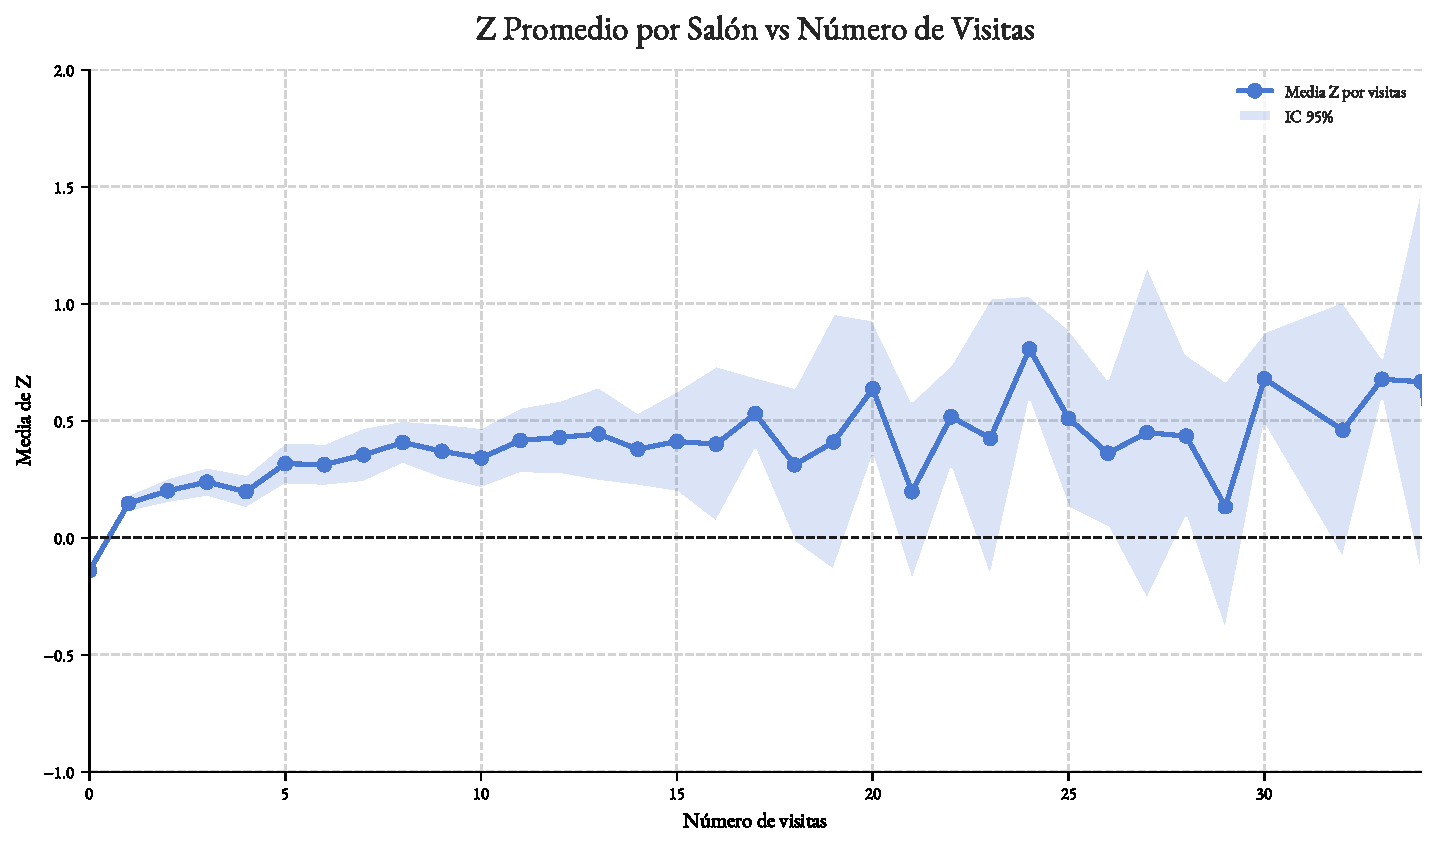
\includegraphics[width=0.7\textwidth,page=1]{09_01.pdf}
    \caption{Z promedio por salón vs número de visitas, con intervalo de confianza del 95\% (IC95\%) alrededor de la media agregada.}
\end{figure}
En la Figura 9.3.1, la media de Z por número de visitas se presenta como una serie agregada acompañada de su IC 95\%.
El PDF no permite distinguir con claridad valores exactos punto a punto, pero sí la escala del eje vertical (media de Z) y el rango de visitas considerado (hasta ~30).
Esta figura está pensada para inspeccionar tendencias promedio con incertidumbre, sin establecer relaciones causales.

\subsection{Intervalos de confianza}
La información de intervalos de confianza para la agregación por visitas está contenida en la Figura 9.3.1 mediante el elemento ``IC 95\%''.
En el PDF no se muestra una tabla de valores; la incertidumbre se expresa visualmente en torno a la media de Z.
En consecuencia, la lectura del IC depende del trazo/banda en la propia figura y de las escalas [-0.5, 1.5] en Z y 0--30 en visitas.


\newpage
\section{Conclusiones}

% Requires: \usepackage{amsmath, amssymb}

\subsection{Contexto y variables}

La variable de resultado es la calificación estandarizada por estudiante,
\texttt{MEAN\_IMPKDE\_Z}. Para cada salón, las calificaciones crudas se
estandarizaron a un Z-score y los valores faltantes se imputaron usando
Kernel Density Estimation (KDE). Por tanto, todos los análisis se realizan
en una escala estandarizada común dentro de cada salón.

Los estudiantes se dividieron en dos grupos según su uso acumulado del CMAT:
\begin{itemize}
  \item \textbf{Grupo A (uso frecuente del CMAT)}: estudiantes con más de tres
        visitas registradas al CMAT ($n_A = 1036$).
  \item \textbf{Grupo B (uso bajo o nulo del CMAT)}: estudiantes con tres o menos
        visitas ($n_B = 9377$).
\end{itemize}

\subsection{Hipótesis}

\textbf{Hipótesis nula:}
\[
H_0:\ \mu_A = \mu_B
\]
Los estudiantes con uso frecuente del CMAT no difieren en su calificación
estandarizada respecto a los estudiantes con uso bajo o nulo.

\textbf{Hipótesis alternativa:}
\[
H_1:\ \mu_A \neq \mu_B
\]
Existe una diferencia en la media de calificaciones estandarizadas entre ambos grupos.

\subsection{Prueba paramétrica}

Se aplicó una prueba $t$ de Welch para comparar calificaciones estandarizadas entre grupos. El resultado fue:

\begin{itemize}
  \item $t = 21.93$
  \item $p < 0.0001$
  \item Media(A) = 0.34
  \item Media(B) = -0.08
  \item Diferencia de medias = 0.41
\end{itemize}

\textbf{Conclusión:} dado que el $p$-valor es esencialmente cero, se rechaza $H_0$.
En promedio, los estudiantes con uso frecuente del CMAT presentan calificaciones estandarizadas mayores.

\subsection{Evidencia robusta (no paramétrica)}

Dado que la distribución no es estrictamente normal, también se aplicaron pruebas robustas. Los resultados fueron consistentes con la evidencia paramétrica:

\begin{itemize}
  \item Mediana(A) = 0.422
  \item Mediana(B) = 0.185
  \item Diferencia de medianas = 0.237 (IC95\% [0.202, 0.284])
  \item Prueba U de Mann--Whitney: $p = 3.224 \times 10^{-50}$
  \item Prueba de Brunner--Munzel: $p = 2.023 \times 10^{-57}$
  \item Tamaño de efecto de lenguaje común: CL = 0.641 (IC95\% [0.625, 0.657])
  \item Correlación biserial por rangos: $r_{rb} = 0.282$ (IC95\% [0.250, 0.313])
  \item Delta de Cliff: $\delta = 0.283$ (IC95\% [0.234, 0.326])
\end{itemize}

\subsection{Cierre}

En conjunto, las figuras y pruebas muestran una separación consistente entre distribuciones de calificación estandarizada para estudiantes con más de 3 visitas al CMAT frente a aquellos con 3 o menos.
La evidencia es observacional: describe asociación y diferencias entre grupos definidos por visitas, pero no establece causalidad.

\end{document}
